% % % Set the style for this file:
\pagestyle{standard}

% % % Beginning of the chapter
\chapter{Preliminary measurements.}\label{chapter3}

	% % % Set the style for the first page:
	\thispagestyle{chapter-first-page}

	\section{Apparent reflected temperature estimation.}\label{section3.1}
	
		In order to correctly estimate the emissivity of any surface, it is very important to determine first the surface apparent reflected temperature. This is crucial, especially for low emissivity materials where a significant contribution is in fact due to the reflected radiation.
		
		A simple method can be used to determine the apparent reflected temperature. To do it, a low emissivity material is needed, usually, an aluminum foil or any other aluminum surface. This method is described as follows:
		
		\begin{enumerate}[label={\arabic*)}]
			\item Place a piece of crumpled and re-flattened aluminium foil in the same position of the object to be measured.
			\item Set the IR camera emissivity internal control to 1.00 and the distance to 0 m.
			\item Point the IR camera to the target (aluminum surface) and select a region of interest (ROI).
			\item Read the value from IR camera on the ROI.
			\item Take the measured value as the apparent reflected temperature.
		\end{enumerate}
	
		Aluminum foil has very low emissivity ($\sim$0.04) and therefore we are certain that almost all IR radiation coming from its surface is reflected from other sources. The camera emissivity is set to 1.00 and the distance to 0 so that the IR camera software does not apply any further correction. The crumpling is done to allow reflections from several directions. For this reason the ROI selected should be as wide as possible since this effect must be averaged out to obtain an accurate estimate of the apparent reflected temperature.\bigskip
	
	\section{Influence of the angular distribution of the emitted IR radiation.}\label{section3.2}
	
		In order to determine whether the viewing angle of the camera with respect to the normal of the petal's surface is a determining factor in our analysis, an study of the angular dependence of emissive power was performed using an aluminum rod filled with hot water placed in the same position as the petal. Using a strip of high emissivity black tape along the rod’s frontal face we were able to measure the variations in temperature due to the viewing angle (Figure \ref{fig3.1}).
	
		\begin{figure}[ht!]
			\centering
			\captionsetup{justification=centering,margin=2cm}
			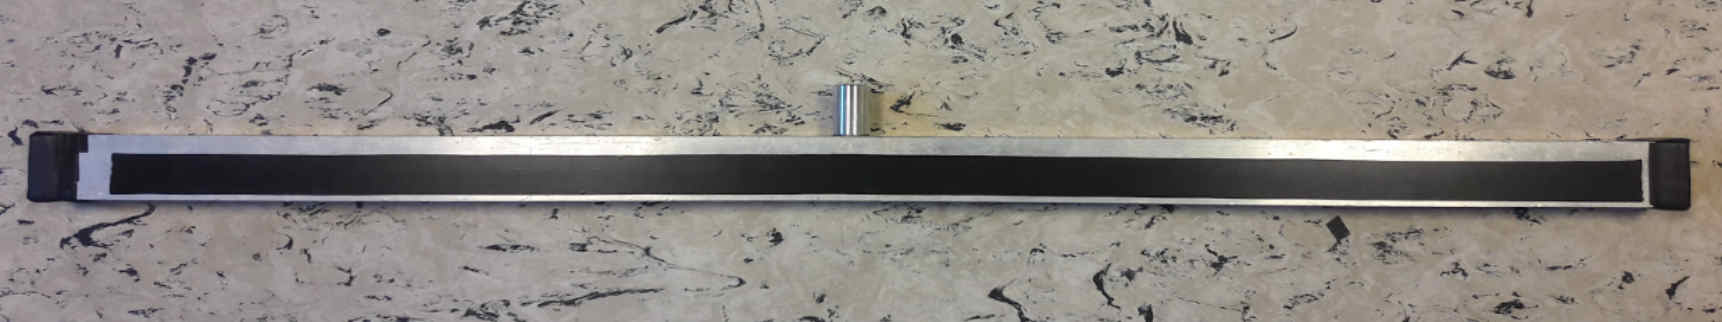
\includegraphics[scale=0.30]{Figures/Chapter03/AluminumRod.jpg}
			\caption{Aluminum rod used to study the angular dependence of emissivity}\label{fig3.1}
		\end{figure}		
	
		A set of measuring areas (ROIs) was defined along the rod using the IR camera software (IRBIS) and a thermocouple was inserted inside the rod in direct contact with the water in order to be able to determine the real temperature of the rod surface. The results can be seen in Figure \ref{fig3.2}. 
		
		We observed that the temperature variations along the rod are within 1$^{\circ}$C, including the error bands, from an angle of 0$^\circ$ (with respect to the normal of the rod’s surface) to roughly 30$^\circ$. For the central values this difference is less than 0.2$^{\circ}$C. This is a relatively small variation for that angular range and even though we see a drop in the markers temperature with respect to the real temperature of 34.6$^{\circ}$C (measured with a thermocouple directly inside the rod) the error magnitude make us conclude that, within this uncertainty, the angle influence on the IR temperature measurements is quite negligible.
		
		\begin{figure}[ht!]
			\centering
			\captionsetup{justification=centering,margin=0cm}
			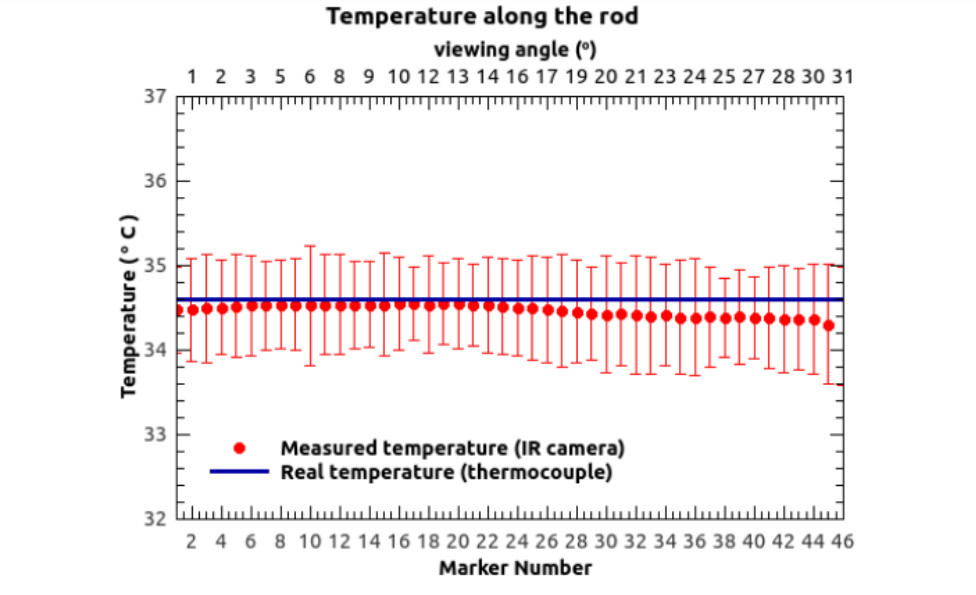
\includegraphics[scale=0.5]{Figures/Chapter03/RodAngularTempResults.jpg}
			\caption{Angle study results using the aluminum rod filled with water at 34.6$^{\circ}$C. The marker positions do not cover the entire rod since it is larger than the petal and some portions fall out of the viewing field of the camera.}\label{fig3.2}
		\end{figure}\bigskip
	
	\section{IR camera spectral response.}\label{section3.3}
	
		From Equation \ref{eq1.16} it can be seen that if we can accurately estimate the emissivity, the apparent reflected temperature and the IR camera spectral response function ($R$) we should be able then to obtain the real temperature of the object for any given spectral power value reported by the camera ($N_{meas}$). 
		
		In order to estimate the $R$ factor we can simply take the emissive power measurements of a surface of known emissivity, the real temperature and the apparent reflected temperature and then use the same Equation \ref{eq1.16} to derive the $R$ scale factor. As this factor only depends on the IR camera, it can be used later on in the analysis as long as we don’t use a different camera.
		For obtaining the scale factor we used an aluminum bucket, which we filled with hot water and recorded the IR power density on several points of the surface (always at the same depth). The measured aluminum surface was coated with high emissivity black\footnote{{\footnotesize Note that the "visible" color of the tape has nothing to do with the emissivity value. It could have been a red, green or even white. The color of the tape is a property related with the visible wavelengths in electromagnetic spectrum while the infrared properties are related with the IR part of the spectrum.}} tape as the water temperature went down to test the temperature dependence of the results (Figure \ref{fig3.3}).
		
		\begin{figure}[ht!]
			\centering
			\captionsetup{justification=centering,margin=2cm}
			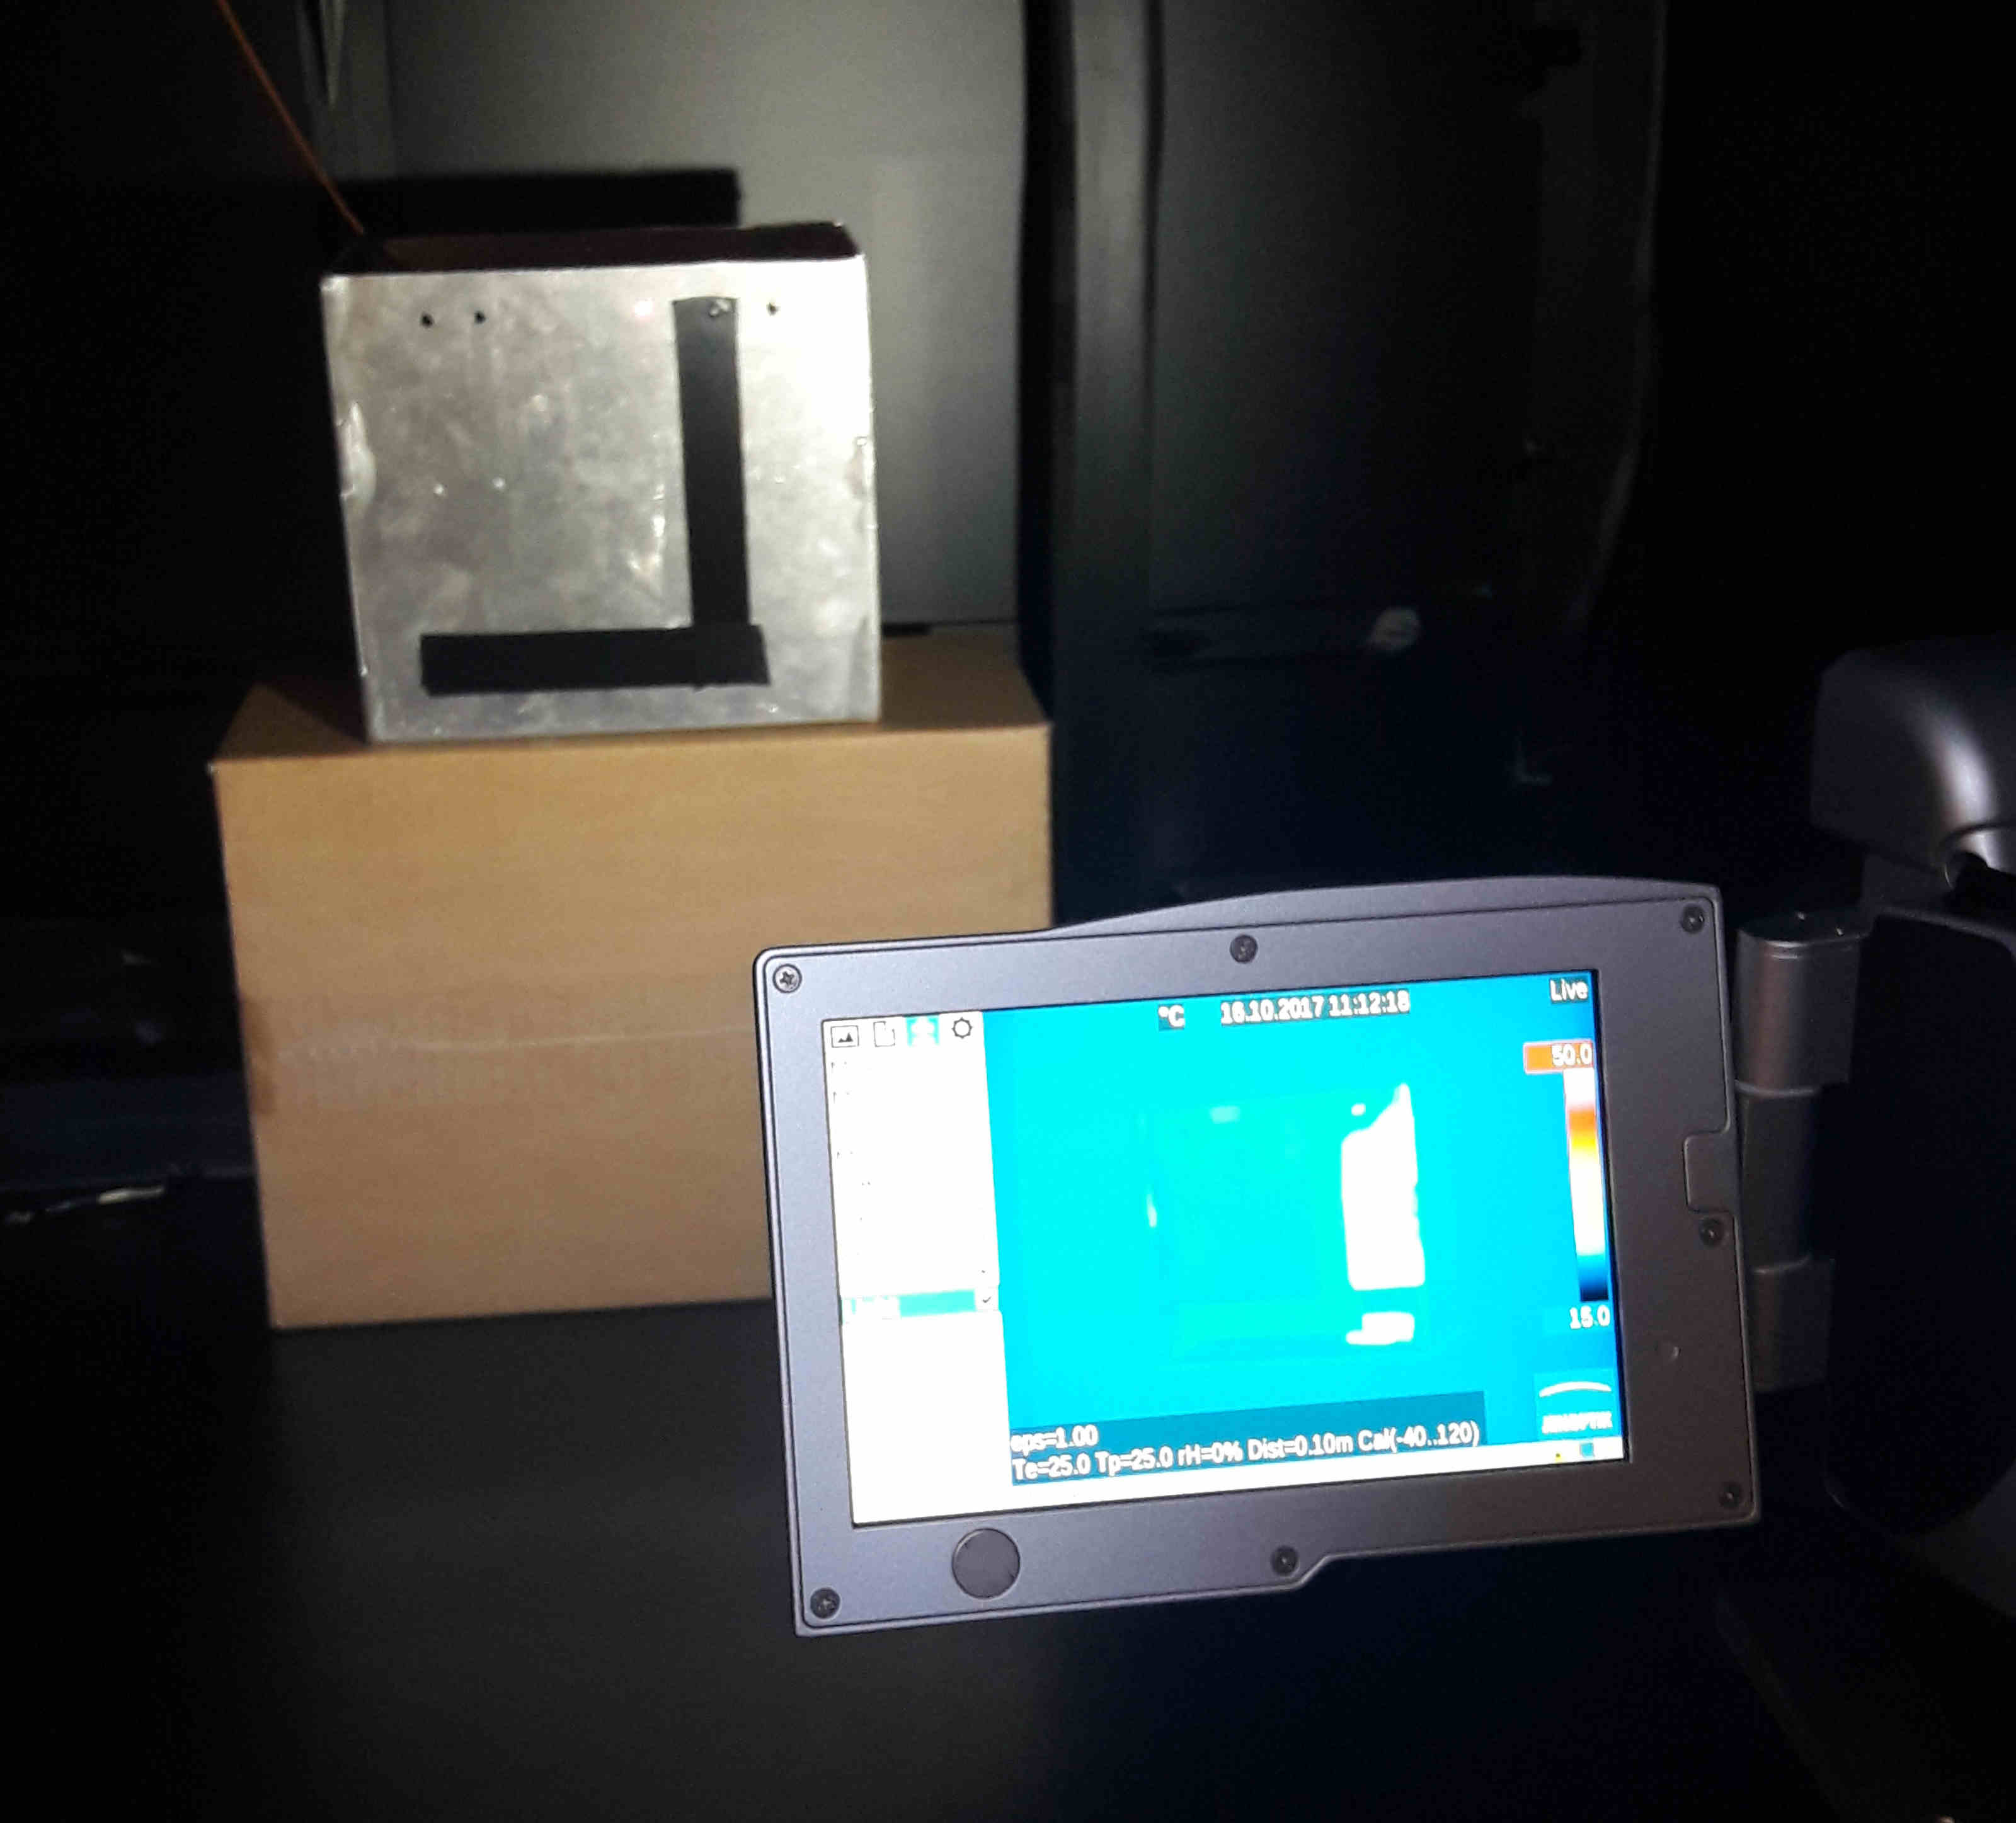
\includegraphics[scale=0.1]{Figures/Chapter03/CameraAndBucket.jpg}
			\caption{Experimental setup to calculate the IR camera spectral response function. Measurements were performed placing measurement markers along the horizontal black tape in the camera IRBIS software.}\label{fig3.3}
		\end{figure}
		
		With this scale factor and Equation \ref{eq1.16} we could estimate the emissivity at pixel level if we had a thermogram in which the real temperature of all the pixels is known. That would allow correct the thermograms in emissivity without the need of covering the Silicon surfaces with high emissivity materials (See Section \ref{section4.1}). That is the so called “baseline image” correction method.
	
		Figure \ref{fig3.4} (left) shows the results of the estimation of the $R$ scale factor for the IR camera using the aluminum bucket filled with hot water. Furthermore, to test the validity of the method we used as well a petal thermogram of which we knew the real surface temperatures, that is, the petal at room temperature without cooling nor electronics powered on. Figure \ref{fig3.4} (right) shows the scale factor estimation on the petal.
		
		\begin{figure}[H]
			\centering
			\captionsetup{justification=centering,margin=2cm}
			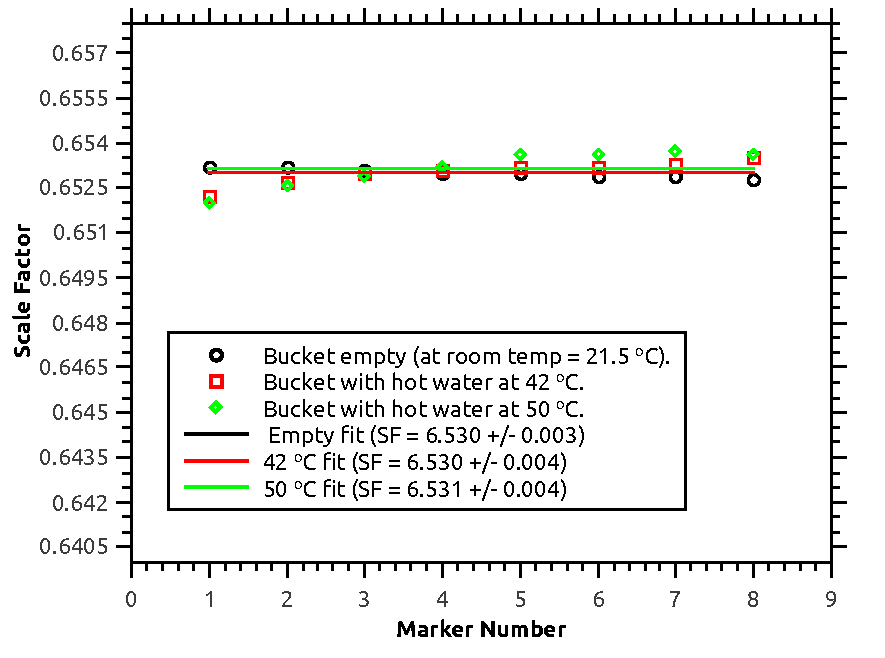
\includegraphics[scale=0.5]{Figures/Chapter03/BucketScaleFactors.pdf}
			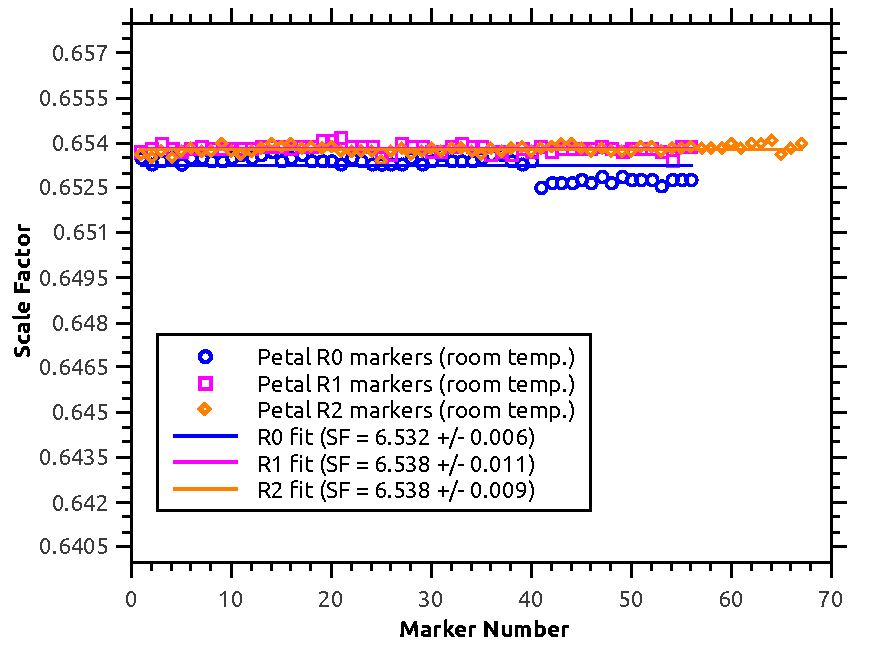
\includegraphics[scale=0.5]{Figures/Chapter03/PetalScaleFactors.pdf}
			\caption{Fits of the IR camera response scale factor calculated for different temperatures using the aluminum bucket (left) and using a petal thermogram (right).}\label{fig3.4}
		\end{figure}
		
		For the calculations, the values of the black tape in silicon modules R0, R1 and R2 were used, showing consistent results with the values obtained with the aluminum bucket. The uncertainty shown is the fit’s root mean squared error. With this test we corroborated that this factor is only dependent on the IR sensor/camera and independent of the temperature and the surface.\bigskip
		
		
		

	